\section{Kerberos delegation}
\label{windows:authentication:kerberos:delegation}
{\bf Kerberos delegation allows a service to access another service on behalf
of the user}

\subsection{Delegation principle}

A web server allows a user to access his personal folder, hosted on a file
server. We are in the following situation :
\begin{figure}
  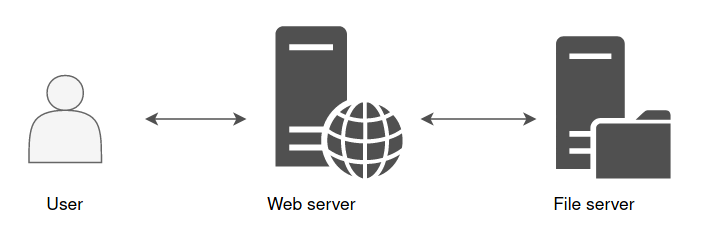
\includegraphics[width=\linewidth]{ad/knowledge/images/webfsuser.png}
  \caption{web fs user}
  \label{fig:webfsuser}
\end{figure}
The web server is front-end, and it’s this web server that will fetch the
information instead of the user on the file server in order to display the
content of a file, for example.

However, the web server does not know what belongs to the user on the file
server. It is not his role to unpack the user’s PAC to make a specific demand
to the file server. This is where the delegation comes in.

This mechanism allows the web server to {\bf impersonate} the user, and to
authenticate on the user’s behalf to the file serve.

from the file server’s point of view, it is the user who makes the request. The
file server will be able to read and check user’s rightsr, then send back the
information to which this account has access.

\begin{figure}
  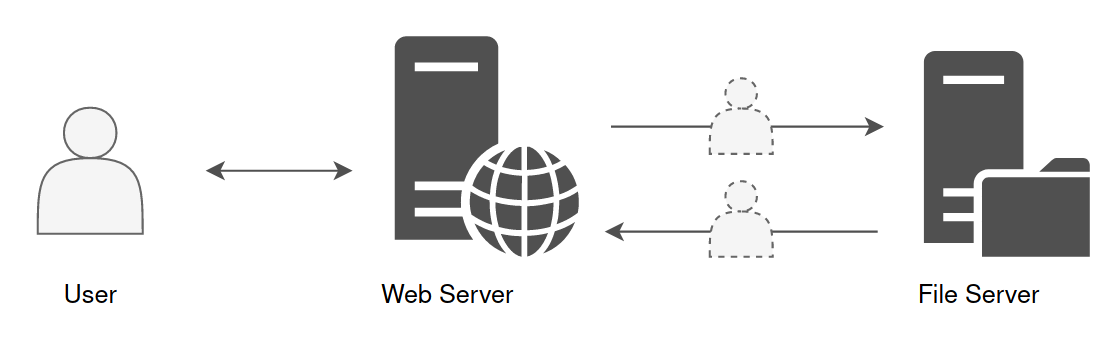
\includegraphics[width=\linewidth]{ad/knowledge/images/impersonation.png}
  \caption{Impersonation}
  \label{fig:impersonation}
\end{figure}


\subsection{Constrained \& Unconstrained Delegation}
The ability to relay credentials can be given to an {\bf account with at least
one SPN attribute set}. It could be a computer account or a service account.

there are three ways to authorize a computer or service account to impersonate
a user in order to communicate with one or more other service(s).

\subsubsection{Unconstrained Delegation}
With Unconstrained Delegation, the server or the service account that is
granted this right is able to impersonate a user to authenticate to {\bf any
services on any host}.



\begin{figure}
  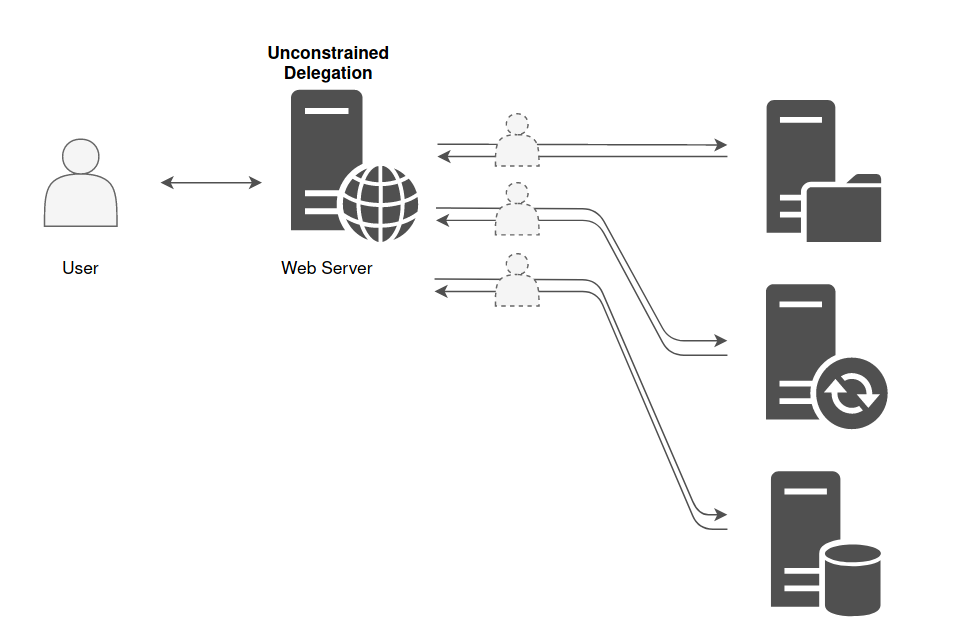
\includegraphics[width=\linewidth]{ad/knowledge/images/unconstrained_delegation_schema.png}
  \caption{Unconstrained delegation}
  \label{fig:unconstrained_delegation_schema}
\end{figure}

\subsubsection{Constrained Delegation}
If a computer or a service account has the Constrained Delegation flag set, a
list of authorized services shall be associated to this flag. 

\begin{figure}
  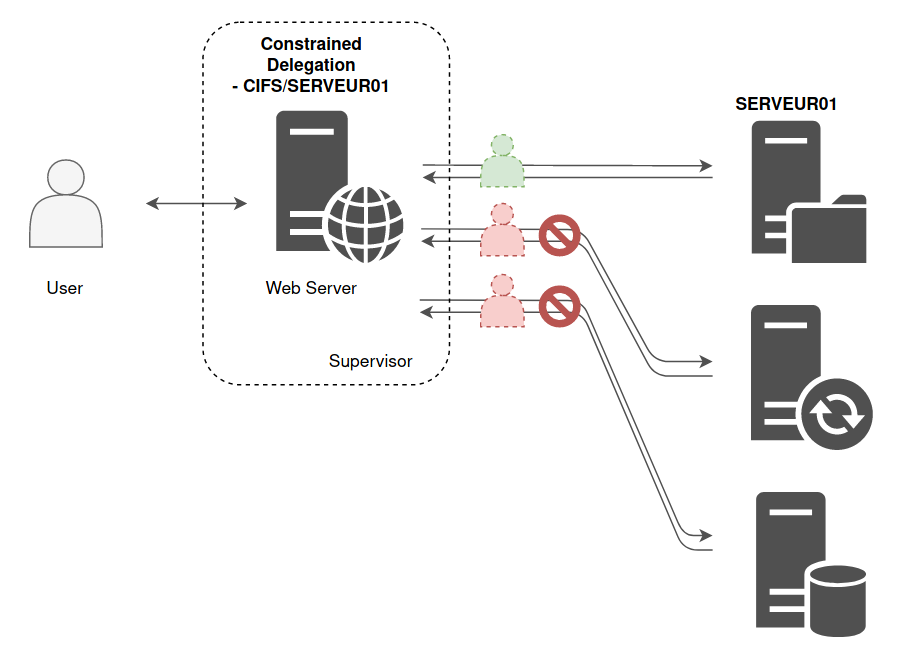
\includegraphics[width=\linewidth]{ad/knowledge/images/constrained_delegation_schema.png}
  \caption{Constrained delegation}
  \label{fig:constrained_delegation_schema}
\end{figure}

\subsubsection{Resource Based Delegation}
In resource based Kerberos delegation, computers (resources) specify who they
trust and who can delegate authentications to them.

This is similar to the basic constrained delegation but instead of giving
permissions to an object to impersonate any user against a service.
Resource-based Constrain Delegation sets in the object who is able to
impersonate any user against it.

Thus, the diagram is as follows :
\begin{figure}
  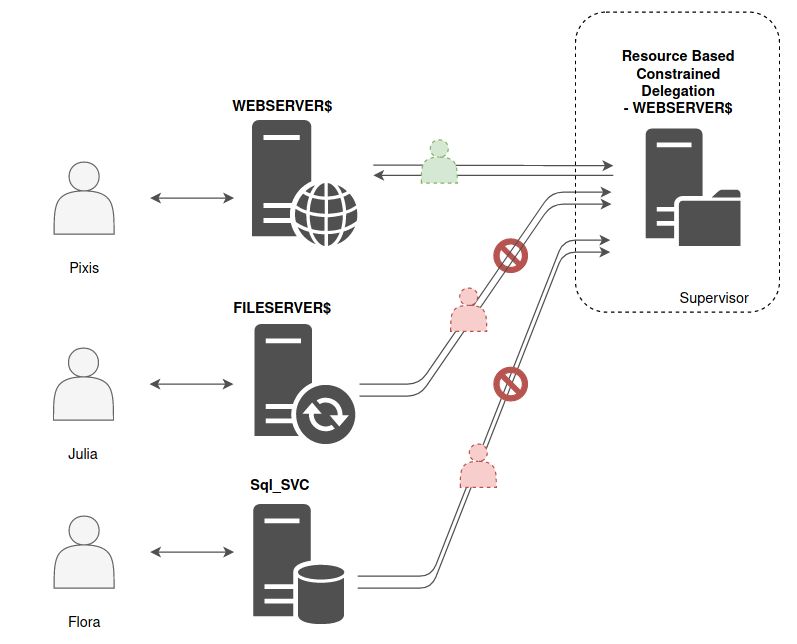
\includegraphics[width=\linewidth]{ad/knowledge/images/resource_based_constrained_delegation_schema.png}
  \caption{iRessource Based delegation}
  \label{fig:resource_based_constrained_delegation_schema}
\end{figure}
The responsibility is shifted, it’s at the level of the resource that receives
the delegated authentications that the information of whether or not the
delegation is accepted is found.

In other words, it’s the end resource that says “I allow this list of accounts
 to authenticate to me on behalf of someone else”.


In this case, the constrained object will have an attribute called
\verb+msDS-AllowedToActOnBehalfOfOtherIdentity+ with the name of the user that
can impersonate any other user against it.

Another important difference from this Constrained Delegation to the other
delegations is that any user with write permissions over a machine account
(\verb+GenericAll/GenericWrite/WriteDacl/WriteProperty/+\ldots) can set the
\verb+msDS-AllowedToActOnBehalfOfOtherIdentity+ (In the other forms of
Delegation you needed domain admin privs).


\url{https://en.hackndo.com/constrained-unconstrained-delegation/}
\subsection{Constrained delegation}

\url{https://book.hacktricks.xyz/windows-hardening/active-directory-methodology/constrained-delegation}
\subsection{Unconstrained delegation}

\url{https://www.secureauth.com/blog/kerberos-delegation-spns-and-more/}
